\startchapter{Evaluation}
\label{chapter:evaluation}

\section{Expert Interface}



\section{Citizen Science Interface}


\section{Distributed Computation}

- Grid Computing
- Mahout


\section{Audio Feature Extraction and Machine Learning}








\section{Old}

\section{Evaluation}

Our evaluation section consists of three parts, in the first we
optimize basic audio feature extraction parameters, in the second we
use different distributed Machine Learning systems to generate
classification results, and in the third we give a report on our
experiences with these different platforms for feature extraction and
Machine Learning.

\subsection{Audio Feature Extraction}

Our first challenge when dealing with the Orchive is the huge size of
the data.  The raw uncompressed .wav files that were digitized from
tape take approximately 12TB on disk at the time of this analysis,
with more files being added all the time.  In order to determine if we
could use a compressed format for doing the audio feature extraction,
we compared the results of using a SVM machine to classify the frames
of audio.  For the original .wav file we got a classification accuracy
of 94.5\%, while a highly compressed 32kbs MP3 gave 93.6\% accuracy.
The disk quota on the Westgrid system is set by default at 1TB, so by
sacrificing a small amount of accuracy, it was possible to reduce the
disk space used from 12TB to 199GB, a 60x savings in space.

In order to test the different distributed audio classification
systems we first generated a set of training and testing data.  In a
previous paper \cite{ness2008}, we were able to obtain a
classification performance of 82\% when using a SVM classifier on hand
labelled data.  While this performance was adequate when used on a
small recording, when run on the entire Orchive, this performance
would lead to way too many false positives.  For this paper, we looked
in more detail at the training data, and found that while the
annotation boundaries were close to the start and end of the
vocalization, there was a small amount of silence before and after the
vocalization.  Using Audacity, we trimmed out all the silences of a 10
second region of audio of orca vocalizations, and did the same to a 10
second region of voice notes.  For the background data, we took one
hundred 0.1 second regions from random background annotations and
joined them together with the Linux audio utility program sox.  The
results for this can be found in the first line of table
\ref{table:handTrimmed} and had over 99.73\% of the instances
classified correctly.  This large jump in performance was unexpected
but easily understood, because if feature vectors of silence are
labelled as orca, this will cause issues for the classifier.  We then
took a 4 minute region of orca calls and voice notes and removed all
the silences from both of them.  We then did a preliminary test where
we reduced computation time by downsampling the feature vectors at a
rate of 100:1, this is shown in the next line of Table
\ref{table:handTrimmed}, and followed this by another test at 10:1
downsampling and one with no downsampling.  These tests gave
classification performance of 95.7\% to 97.7\%.  We then repeated the
analysis in our previous paper by using non-hand-trimmed audio, the
results are shown in the third section of the table.  We found results
from 88.1\% to 93.0\% for 100:1 and no downsampling.  The difference
of this result from the previous paper is likely due to the exact
training and testing sets used in the two papers.  In the current
paper, we are classifying only nearby and isolated orca vocalizations
and not the distant or noisy vocalizations, which was a small tweak to
the experimental setup that has also helped us to not only achieve
better classification performance but to deliver a science goal more
pertinent to the bioacoustics researchers who could use the Orchive.

\begin{table}
\begin{tabular}{|l|c|l|l|r|r|}
\hline
 trim & time (min)  & ds & features & \# & \% corr.  \\
\hline
 x & 10 sec  &  1   & all   &    2586  &    99.73  \\
\hline
 x & 4       & 100  & all   &     606  &    95.71  \\
 x & 4       & 10   & all   &    6060  &    97.19  \\ 
 x & 4       & 1    & all   &   60596  &    97.72  \\
 x & 4       & 100  & mfcc  &     606  &    94.88  \\
 x & 4       & 10   & mfcc  &    6060  &    96.03  \\
 x & 4       & 100  & yin   &     606  &    xx.xxxx  \\
 x & 4       & 10   & yin   &    6060  &    xx.xxxx  \\
\hline
   & 4       & 100  & all   &     621  &    88.08  \\
   & 4       & 10   & all   &    6202  &    92.26  \\
   & 4       & 1    & all   &   62023  &    93.01  \\
   & 4       & 100  & mfcc  &     621  &    87.76  \\
   & 4       & 10   & mfcc  &    6202  &    91.52  \\
\hline
\end{tabular}
\caption{Classification results with hand trimmed orca vocalizations
  using bextract to generate audio features and the SVM classifier in
  Weka to do a 10-fold crossvalidation of these features.}
\label{table:handTrimmed}
\end{table}

The next task that we worked on was to determine the optimal settings
for the audio extraction algorithm.  While there are a number of other
audio extraction frameworks in existence like jMIR \cite{mckayphd},
SmIrK \cite{wang07} and AIMC \cite{waltersphd}, the Marsyas framework
implements most, if not all, of the most popular audio feature
extraction algorithms, and presents them as output from the
``bextract'' program as .arff files, which are the input to the Weka
suite of Machine Learning programs.  For all experiments here, we use
the audio features calculated by Marsyas, however in the future it
would be desirable to integrate other audio processing frameworks
within OpenMIR.

The features output by bextract include the number of zero crossings
per unit time, three spectral descriptors (centroid, rolloff, flux),
Mel-Frequency Cepstral Coefficients (MFCC) and chroma information
based on the western equally tempered scale.  The mean and standard
deviation of each of these over a window is then calculated and forms
the output.  The first experiment we did was to determine if the MFCC
coefficients contained enough information to do the classification on
their own, the results for this are shown in Table
\ref{table:handTrimmed} in the columns with ``mfcc'' in the
``features'' column.  For the hand trimmed example at a downsampling
of 10:1, the performance goes from 97.2\% to 96.0\% which is a small
but meaningful difference, especially when one considers how many more
false positives one would get when looking at the entire Orchive.  We
also tried adding the Yin pitch estimator as another feature in the
feature vector output by bextract.  Surprisingly, as one can see in
the previous table, the addition of this information actually degraded
performance of the classifier.  We are currently investigating how to
better incorporate pitch tracking information in our classifiers.

The next set of parameters that needed to be optimized were the Window
Size and Hop Size of the Digital Signal Processing (DSP) algorithms
that take the input audio and calculate spectral information from
them, the fundamental basis for which is the Fast Fourier Transform
(FFT) algorithm.  One other important input to the bextract feature
extraction algorithm is the length of time over which to calculate the
statistical properties of the features, this is known in bextract as
the ``memory'' and corresponds to the number of frames of features
that are accumulated.  The results for this are shown in Table
\ref{table:dspParams}.  From this we can see that as we go to longer
window sizes, the classification performance increases, and as we go
to longer accumulation window sizes, the performance also increases.

For our experiments we decided that a good sweet spot was a hop size
size of 1024 and a memory of 40 frames, which gave a classification
performance of 99.7\%.  80 frames of audio at a sampling rate of 44100
samples/sec and a hop size of 1024 would result in a feature length of
1.86 seconds, while 40 frames would only give 0.93 seconds of audio
per feature.  Given that orca vocalizations are usually between 0.5
and 3 seconds long, we chose a window size of 2048, a hop size of 1024
with an accumulator memory of 40 frames.  We did extensive experiments
with other values of hopsize, window size and memory that were
consistent with these results that are too long to report here.

\begin{table}
\begin{tabular}{|r|r|r|r|r|r|}
\hline
 winsize  &  hopsize  &  memory  &  total &   correct  \\
\hline
     256  &      128  &      20  &        13767   &    97.11  \\
     512  &      256  &      20  &        11647   &    96.11  \\
    1024  &      512  &      20  &         5923   &    97.74  \\
    2048  &     1024  &      20  &         2995   &    98.84  \\
\hline
     256  &      128  &      40  &        23311   &    96.18  \\
     512  &      256  &      40  &        11829   &    97.61  \\
    1024  &      512  &      40  &         5991   &    98.86  \\
    2048  &     1024  &      40  &         3022   &    99.74  \\
\hline
     256  &      128  &      80  &        23628   &    97.48  \\
     512  &      256  &      80  &        11963   &    98.71  \\
    1024  &      512  &      80  &         6044   &    99.74  \\
    2048  &     1024  &      80  &         3027   &    99.90  \\
\hline
\end{tabular}
\caption{DSP parameters}
\label{table:dspParams}
\end{table}

\subsection{Machine Learning}

The main distributed Machine Learning framework we used was Mahout,
which as we previous described is a Java framework for Machine
Learning that operates on top of Hadoop.  We investigated a number of
its algorithms and found that the Logistic Regression algorithm was
the only classification algorithm that was both suitable for our
problem and incorporated into the main source code trunk of the code.
Our first experiment was just to test the two parameters suggested for
tuning this algorithm are shown in Table
\ref{table:logisticRegressionTests}, and from these brief experiments
it appears the default parameters work best on this data.

\begin{table}
\begin{tabular}{|r|r|l|}
\hline
 Passes  & Rate  & Percent Correct                                         \\
\hline
    100  &    50  &  85.5  \\
   1000  &    50  &  85.5  \\
    100  &     5  &  83.0  \\
    100  &   500  &  85.5  \\
\hline
\end{tabular}
\caption{Logistic regression tests with different parameters.}
\label{table:logisticRegressionTests}
\end{table}

We then took a randomly selected 13GB portion of the 500GB of total
(one of the original 37 shards from feature extraction) audio features
calculated in the previous section and ran a comparison of the Mahout
Logistic Regression algorithm against a simple parallel
implementation using a script that runs Weka jobs on multiple
computers using the Torque/PBS system on the Westgrid cluster.

For this we had our choice of a number of systems on which to run a
Mahout/Hadoop cluster on and investigated all of them.  The first was
Emulab, which is a fine platform and is very useful for a number of
use cases, but for this case of obtaining 10-20 computers and storing
substantial amounts of long lived data on them did not fit the Emulab
model of running distributed programs on different types of emulated
networks on short lived borrowed computers.  While it would have been
possible to use Emulab, we were hoping for a longer term solution.
Planetlab allows for longer leases, but the large memory and CPU
requirements of our program made this less feasible as well.  We
attempted to obtain machines on the GeniCloud at HP, but were unable
to obtain the machines in the end.  The best solution we felt was to
use the six GreenGeni nodes at UVIC and setup a Hadoop cluster on
these.  We attempted to do this for quite some time, but ran into a
number of odd port issues.  We suspect the problem are concurrently
running Swift and Disco installs on these machines that might be
utilizing these ephemerally used ports.  The problem could also be due
to a misconfiguration of the networking hardware.  Another solution
would be to use the Amazon EC2 cluster service, or even their Elastic
MapReduce service, a service that is easy to setup and use, however,
costs for it can add up quickly.  For the results in this paper we use
a mini 2-node Hadoop cluster that was setup in our lab in a controlled
setting, this was simple to install and get results from.  In the near
future we hope to setup a larger Hadoop cluster and to rerun these
jobs with more processors.

For all of our analysis here, we took one of the 37 splits of the
original data analyzed by bextract.  This file was 13GB in size and
contained 22486467 lines.  For the following experiments we took the
first $n$ lines of this file where $n$ started at 10 and increased to
10,000,000 in powers of 10.

For the first experimental condition, the Logistic Regression
Classifier as implemented in Mahout was used, and Hadoop was used as
the underlying system below Mahout.  The Logistic Regression
classifier as implemented by default in Mahout can only take two
classes as input, so for all these experiments we used only orca and
background as the training data.  The timing results of Logistic
Regression in Mahout are shown in Table
\ref{table:machineLearningTiming1}.  As we can see, the system is very
fast, even classifying a million instances only takes one minute on a
small two node cluster.  As the number of instances increases, the
time increases quickly, it would be interesting to see this with a
larger cluster of 10 or more nodes.

For the second experimental condition, we used the Weka Machine
Learning package and ran it with it's Logistic Regression engine.
This was run on the Hermes cluster at Westgrid, and for these tests,
only 10 nodes were run at one time, although scaling up is as simple
as splitting the input file into more chunks and starting more jobs.
Weka is a Java program, and thus incurs a certain startup time when
creating and setting up the JVM and other resources.  This is
reflected in the results in Table \ref{table:machineLearningTiming2}
where up to 100000 instances the run times are all around 6 seconds.
The third experimental condition was to use Weka again, but this time
with its SVM engine.  Interestingly, the time that the SVM took to run
was about the same as the Logistic Regression, even though SVM is
typically be a considerably better classifier than Logistic
Regression.

In the final experiment, PSVM was run on the Checkers cluster at
Westgrid.  It was unable to be run on the Hermes and Nestor clusters
due to the use of MPICH2 by PSVM and the use of the original MPI
version 1.0 on the clusters.  This program takes advantage of the MPI
message passing library to communicate between a number of different
computers, and for the experiments shown below, we used 4 processors.
It should be noted that at least on the Checkers cluster, it is
difficult to reserve a block of 5 computers at once, much more
difficult than starting 5 individual jobs.  Depending on the cluster
you have access to, this may or may not be a problem.


\begin{table}
\begin{tabular}{|l|r|r|r|}
\hline
 system  &  \# proc.  &  num instances  &  time (sec)  \\
\hline
 Mahout  &     2          &            100  &       0.55  \\
 Mahout  &     2          &           1000  &       0.89  \\
 Mahout  &     2          &          10000  &       1.45  \\
 Mahout  &     2          &         100000  &       6.69  \\
 Mahout  &     2          &        1000000  &      57.90  \\
 Mahout  &     2          &       10000000  &     566.35  \\
 Mahout  &     2          &       22486467  &     566.35  \\
\hline
 PSVM     &           10  &            100  &     2  \\
 PSVM     &           10  &           1000  &     1  \\
 PSVM     &           10  &          10000  &     1  \\
 PSVM     &           10  &         100000  &     50  \\
 PSVM     &           10  &        1000000  &     635  \\
 PSVM     &           10  &       10000000  &       \\
 PSVM     &           10  &       22486467  &       \\
\hline
\end{tabular}
\caption{Timing results for all Machine Learning Algorithms}
\label{table:machineLearningTiming1}
\end{table}

\begin{table}
\begin{tabular}{|l|r|r|r|}
\hline
 system  &  \# proc.  &  num instances  &  time (sec)  \\
\hline
 Weka : LogReg    &           10  &            100  &        6.03  \\
 Weka : LogReg    &           10  &           1000  &        6.05  \\
 Weka : LogReg    &           10  &          10000  &        6.09  \\
 Weka : LogReg    &           10  &         100000  &        7.55  \\
 Weka : LogReg    &           10  &        1000000  &       31.24  \\
 Weka : LogReg    &           10  &       10000000  &      183.74  \\
 Weka : LogReg    &           10  &       22486467  &      233.99  \\
\hline
 Weka : SVM     &           10  &            100  &        5.38  \\
 Weka : SVM     &           10  &           1000  &        5.35  \\
 Weka : SVM     &           10  &          10000  &        5.15  \\
 Weka : SVM     &           10  &         100000  &        7.53  \\
 Weka : SVM     &           10  &        1000000  &       28.66  \\
 Weka : SVM     &           10  &       10000000  &      182.61  \\
 Weka : SVM     &           10  &       22486467  &      	  \\
\hline
\end{tabular}
\caption{Timing results for all Machine Learning Algorithms}
\label{table:machineLearningTiming2}
\end{table}


\section{Orca}

\begin{table}
\caption{Classification Performance}
\begin{tabular}{|c|c|c|} \hline

Dataset&Correctly Classified Instances&Percent Correct\\ \hline

446A & 30403 & 90.31\\ \hline
446B & 33701 & 81.97\\ \hline
447B & 23013 & 73.65\\ \hline
448A & 15307 & 58.04\\ \hline
448B & 20822 & 74.61\\ \hline
449B & 25239 & 81.17\\ \hline
450A & 31872 & 87.85\\ \hline
450B & 23916 & 93.51\\ \hline
451A & 54281 & 89.74\\ \hline
451B & 25528 & 69.91\\ \hline
\hline\end{tabular}
\end{table}



\begin{table}
\centering
\caption{Recording-specific classification performance}
\begin{tabular}{|c|c|c|c|c|} \hline

&\multicolumn{2}{|c|}{Naive bayes}&\multicolumn{2}{|c|}{SMO}\\
&\multicolumn{2}{|c|}{\% correct}&\multicolumn{2}{|c|}{\% correct}\\ \hline
&self&train with&self&train with\\
&&remaining&&remaining\\ \hline

446A  &  89.42  &  93.10  &  95.00  &  73.39\\ \hline
446B  &  63.45  &  77.66  &  85.85  &  70.23\\ \hline
447B  &  75.46  &  57.32  &  82.02  &  68.17\\ \hline
448A  &  52.18  &  61.02  &  81.57  &  62.24\\ \hline
448B  &  84.63  &  67.62  &  83.64  &  67.87\\ \hline
449B  &  82.24  &  51.85  &  86.41  &  75.72\\ \hline
450A  &  94.66  &  90.91  &  96.12  &  91.58\\ \hline
450B  &  83.65  &  96.27  &  99.29  &  94.92\\ \hline
451A  &  70.92  &  89.58  &  97.04  &  78.72\\ \hline
451B  &  74.18  &  33.73  &  82.34  &  50.88\\ \hline
\end{tabular}
\label{table:classification}
\end{table}


In order to explore whether this idea would work for our data, we 
created a representative database consisting of 10 excerpts from 
our recordings with each excerpt lasting between 5 and 10 minutes. 
Table ~\ref{table:classification} shows classification results using 
10-fold cross-validation for each particular recording using a
recording specific classifier as well as using a classifier trained 
on the entire dataset. Two classifiers are used: a simple Naive Bayes
classifier (NBS), as well as a Support Vector Machine (SVM). The results shown 
are based on the use of the standard Mel-Frequency Cepstral
Coefficients (MFCC) as audio features. The ``self'' column shows the 
classification accuracy results of using a recording-specific
classifier, whereas the ``remaining'' columns 
shows the classification accuracy results using the remaining nine
recordings. As can be seen, recording-specific classifier can generate
significantly better results than generalized classifiers, which is not 
surprising as they adapt to the specific data of the recording. This
justifies the use of their annotation results to labeled the unlabeled 
parts of the audio recording. 


In order to systematically explore the different strategies for Orca
call retrieval we utilized a dataset consisting of 185 recordings of
vocalizations. They have been annotated using the Orchive
collaborative user interface and classified into 4 discrete call types
by volunteers. The ground truth labels have been verified by
experts. Table ~\ref{table:dataset} shows the composition of the
dataset used for evaluation. We use two established evaluation metrics
that measure the retrieval effectiveness. Precision at 1 is simply the
number of queries for which the first retrieved call has the same
class as the query. The mean average precision (MAP) is the most
frequently used summary measure of a ranked retrieval run. Average
precision of a single query is the mean of the precision scores after
each relevant document has been retrieved. The value for the run (a
set of queries) is the mean of the individual average precision
scores. MAP combines aspects of both precision and recall and rewards
returned relevant items higher in the list.


\begin{table} 
\begin{center}
\caption{Dataset composition and MAP scores for best configuration
  (Hertz frequency scale, SACF pitch extractor and DTW matching) } 
\begin{tabular}{|l|c|c|c|c|}
\hline
Call Type     & N1      & N3      & N4 & N47 \\ 
\hline 
Instances     & 36      & 56      & 60  &  33 \\ 
\hline 
MAP            & 0.63   &  0.94   & 0.78  & 0.58  \\ 
%  Precision@1 &      &       &      &       \\ 
\hline 
\end{tabular} 
\label{table:dataset}
\end{center}
\end{table} 


Table ~\ref{table:dataset} shows the best MAP scores achieved for each
type of call. As can be seen there is large variance in the MAP score
for different types of calls. For example retrieval of N3 calls is
very robust but retrieval of the N47 calls is not as much. These
differences are also observed in the human classification of these
calls. 

Table ~\ref{table:dataset_map} shows the MAP scores and
average precision score at 1 over the entire dataset for combinations
of different representations and pulse rate extraction strategies. As
can be seen, the SACF pitch extractor is the best performing pitch
extraction method independently of the retrieval strategy. The DTW
matching is also the best performing retrieval strategy. It is hard to
draw any conclusions with respect to SACF performing better than the
other two pitch extractors. The better results obtained using the DTW
retrieval strategy indicate there is important non-uniform timing
variation in the structure of these calls. 

We have also conducted experiments with different frequency scale
representations such as the Bark-scale \cite{zwicker1961} and
logarithmic frequency but in all configurations they performed worst
than the default linear frequency representation in Hertz.



\begin{table} 
\begin{center}
\caption{Mean Average Precision Scores for different pitch extraction 
and retrieval strategies} 
\begin{tabular}{|l|c|c|c|}
\hline   
              & Features           & Contour & DTW \\
\hline 
PRAAT     & 0.38       & 0.52         & 0.67 
   \\ 
\hline 
YIN          & 0.50        & 0.51         & 0.72  \\ 
\hline 
SACF        & 0.63     & 0.66          &  0.77 \\ 
%  Precision@1 &      &       &      &       \\ 
\hline 
\end{tabular} 
\label{table:dataset_map}
\end{center}
\end{table} 


\begin{table} 
\begin{center}
\caption{Average Precision at 1 scores for different pitch extraction 
and retrieval strategies} 
\begin{tabular}{|l|c|c|c|}
\hline   
              & Features & Contour & DTW \\
\hline 
PRAAT     &    0.38      &       0.40       &  0.4      \\ 
\hline 
YIN          &    0.77         &   0.72          &       0.95 \\ 
\hline 
SACF        &    0.79   &    0.82    &  0.95 \\ 
%  Precision@1 &      &       &      &       \\ 
\hline 
\end{tabular} 
\label{table:dataset_prec1}
\end{center}
\end{table} 


\begin{table}
\begin{tabular}{|l|l|l|l|}
top-k & SAI & MFCC & percent error reduction \\ \hline
1 & 27 & 33 & 18 \% \\
2 & 39 & 44 & 12 \% \\
5 & 60 & 62 & 4 \% \\
10 & 72 & 74 & 3 \% \\
20 & 81 & 84 & 4 \% \\
\end{tabular}
\caption{A comparison of the best SAI and MFCC configurations.  This
  table shows the percent error at top-k, where error is defined as 1
  - precision.}
\label{table:topk}
\end{table}

\begin{table}
\centering
\begin{tabular}{|l|l|}
Algorithm & Classification Accuracy \\\hline
SAI/VQ & 0.4987 \\
Marsyas MFCC & 0.4430 \\
Best & 0.6526 \\
Average & 0.455 \\
\end{tabular}
\caption{Classical composer train/test classification task}
\label{table:classical}
\end{table}

\begin{table}
\centering
\begin{tabular}{|l|l|}
Algorithm & Classification Accuracy \\\hline
SAI/VQ &  0.4861 \\
Marsyas MFCC & 0.5750\\
Best &  0.6417 \\
Average &  0.49 \\
\end{tabular}
\caption{Music mood train/test classification task}
\label{table:mood}
\end{table}

\section{Bird}


There are three main areas that we investigate in this work.  The
first is to determine which of the approximately 22,000 recordings in
the Orchive contain acceptably low levels of boat noise.  The second
is to pull out individual clips of orca vocalizations from these
quieter recordings.  The third task is to classify these individual
vocalizations into call classes according to classes previously
identified by whale researchers.

In this work we subdivide our work into three sections, in the first,
we classify whole recordings into ``silent'' and ``noisy'', in the
second we segment the audio recording into ``background'', ``orca'',
and ``voice note''.  In the third we classify small clips of known
orca vocalizations into different call types, as identified in a
pre-existing orca call catalog.

\subsection{Silent and Noisy recordings}

To classify whole recordings into the classes silent and noisy, we
first collected a set of 100 examples of silent recordings, and a set
of 100 examples of noisy recordings.  We then extracted audio features
from these recordings and output these as a .arff file.  This file was
then processed with the SMO SVM classifier in Weka to generate the
classification accuracy numbers shown in the next section.  To
classify recordings, we extracted audio features from each clip of an
audio file which were output as a .arff file and used a C++ program
that used libSVM to classify each 1 second clip of the audio file.

\subsection{Orca, Voice Note, Background}

To segment recordings into Orca, Voice Note and Background, we used a
C++ program that combined an audio feature extraction engine with an
SVM classifier. We trained this classifier on different amounts of
data and evaluated the performance of each of the resulting Support
Vector Machines.  The C++ program classified each frame of audio
features into a class, and then performed a neighborhood voting
scheme, where a 1 second window of multiple 20ms frames were used, and
the class that had the most number of frames that were classified as
that class was output.  For example, if 80 frames were classified as
orca, 15 as voice and 5 as background, the classifier would output
``orca 80'' for that 1 second section of audio.

\subsection{Orca call classification}

In order to classify orca calls according to a pre-defined call
catalog, 325 clips containing orca vocalizations were classified by
hand into six classes of common calls, which were ``N1'', ``N3'',
``N4'', ``N7'', ``N9'' and ``N47''.  A single audio feature vector for
each clip was calculated which contained the mean and standard
deviation for the audio features mentioned above.  This gave a feature
vector of size 68 which was output in .arff format.  These files were
then used as input to Weka and three different classifiers were used,
including J48, Naive Bayes and the SMO SVM classifier.

\section{Results}\label{sec:results}

\subsection{Audio Feature Extraction}

We did a parameter search over window size, hop size and memory size.
The results of this are shown in Table \ref{table:afe}.  From this
table we can see that the optimal setting of window size and hop size
is 2048 and 1024 and the optimal window size is 40 frames.  While it
would be possible to go to large window sizes, in our experience this
blurs out the frequency to an unacceptable level in other Machine
Hearing tasks and makes segmentation of the audio problematic.

\begin{table}
\centering
\caption{Audio Feature Extraction}
\begin{tabular}{ccccc} 
\hline
Window Size & Hop Size & Memory & \% correct & \# data points \\  \hline
\\ 
1024 & 512  & 1  & 83.5 & 282899 \\
1024 & 512  & 10 & 87.7 & 282899 \\
1024 & 512  & 40 & 92.5 & 282899 \\
2048 & 1024 & 1  & 84.1 & 143049 \\
2048 & 1024 & 10 & 91.3 & 143049 \\
2048 & 1024 & 40 & 93.7 & 143049 \\
\\ \hline
\end{tabular}
\label{table:afe}
\end{table}


\subsection{Silent and Noisy recordings}

As training data for this task, we labeled 100 instances of audio as
``silent'' and 100 instances of ``not-silent'' and extracted a variety
of audio features from these files, including MFCC coefficients,
general spectral descriptors such as the centroid frequency, Rolloff
frequency and flux, and the number of zero crossings per window.

For this experiment, we extracted a single summary vector for each
audio clip containing 68 elements, which were the mean and standard
deviation for each of the audio features given above.  We generated
audio features for these 200 instances and classified them using the
SMO SVM classifier in Weka.  From this we obtained a classification
accuracy of 82.5\%.

To provide a summary of the recordings in the Orchive, 6 clips of 1
second in duration were extracted from each recording.  This gave a
total of 125,347 clips, totaling 2089 hours of audio.  We extracted
the same features as those extracted from the training data above and
output these vectors as a .arff file.  These vectors were then used as
training data for an SVM classifier implemented in C++ and using
libSVM \cite{cc01} as the classifier. We took each of the 125,347
clips of audio and classified each one of them into the classes
``noisy'' and ``silent''.  Of these, 87,657 were classified as noisy
and 37,690 were classified as quiet.  The quiet recordings would
provide for a good dataset for researchers to examine first, and could
then move on to progressively more difficult recordings as their
research project required more data.

\subsection{Orca, Voice Note, Background}

As an initial study, a total number of 3265 samples of data labeled
with ``orca'', ``voice'' and ``background'' was used to train a Naive
Bayes classifier in Weka with default parameters.  This gave a
classification accuracy of 68.3\%.  The same data was also used to
train a SVM using the SMO classifier in Weka with default parameters
which gave a classification accuracy of 77.6\%.  The confusion matrix
is shown below.

\begin{verbatim}
    a    b    c   <-- classified as
  886  298    2 |    a = b
  376 1516    3 |    b = o
   34   17  133 |    c = v
\end{verbatim}

It can be seen from this confusion matrix that background and orca
vocalizations are labeled as each other quite often.  In the Orchive,
the majority of the audio data is of background recordings, and an
important task is for the machine learning system to distinguish
background recordings from orca vocalizations.  If our classifier
gives a large number of false positives, it will be difficult for
researchers to use this data to find orca vocalizations.

Upon further examination it became clear that the problem was that the
large amount of background noise in the recordings was difficult for
our chosen audio features.  It was then decided to instead train a
classifier to identify clearly identifiable orca vocalizations, and
then extract these clear vocalizations from the archive for further
processing.  From the results of the previous section, where we
identified a large number of recordings with silence in them, this
limited amount of data would still represent a large dataset to study.

To improve classification accuracy, a set of 725 audible orca recordings
was chosen using the orcaGame interface.  534 clear voice recordings
were also collected, and 1539 background recordings were collected.
We then randomized selected subsets of 10, 50 and 500 recordings from
each of these collections and trained a machine learning classifier on
each of these collections.  To test these classifers, we used a
separate set of recordings, and used a neighbourhood voting method,
where each 20ms section of audio was classified by a SVM classifier,
and then the results of 1 second of these were collected.  The scheme
we used is described in the Data Mining section above.

The results from this are shown in Table \ref{table:obv}.  From this
we can see that the classification performance for classifying orca,
background and voice is approximately 85\%-89\%.  We are currently
running this classifier on all recordings in the Orchive, but due to
it's slow speed, are looking for ways to downsample this data and
provide a performance boost.


\begin{table}
\centering
\caption{Orca / Background / Voice}
\begin{tabular}{cccccc} 
\hline
\# Training & Time & Time to classify & \% correct & \% background & \% voice  \\  
samples & to train & classify 1 sec & orca & background & voice \\ \hline
\\ 
150   & 525    & 0.1 sec  & 64.1 \%  & 46.7 \%  & 91.7 \% \\
300   & 2103   & 0.5 sec  & 79.6 \%  & 66.0 \%  & 93.5 \% \\
1500  & 29025  &   2 sec  & 84.6 \%  & 85.3 \%  & 88.9 \% \\
\\ \hline
\end{tabular}
\label{table:obv}
\end{table}


\subsection{Orca call classification}

Using the Orchive and orcaGame web interfaces, we created a collection
of 319 calls of 6 classes, these included the common calls ``N1'',
``N3'', ``N4'', ``N7'', ``N9'' and ``N47''.  Audio features for each
20ms audio frame of these files were generated, these included the
MFCC coefficients, Centroid, Rolloff, Flux and Zero crossings.  The
mean and standard deviation for each of these features were then
calculated and were output as a .arff file.  

These were then classified with Weka using the J48 tree classifier,
which gave an accuracy of 58\%.  We next tried the Naive Bayes
classifier which gave an accuracy of 64.6\%.  The SMO SVM classifier
produced the best results, giving an accuracy of 75.9\%.

The confusion matrix for the SVM classifier is shown below.  From this
we can see that most of the classes are classified correctly.  One
interesting point is that there is some confusion between the N7 and
N9 calls, and it can be noted that these calls are often confused with
each other by humans as well.

\begin{verbatim}
 a  b  c  d  e  f   <-- classified as
 30  0  0  1  0  4 |  a = N1
  1 53  2  0  0  0 |  b = N3
  0  1 80  9  1  2 |  c = N4
  0  0 32  0  0  1 |  d = N47
  0  2  1  0 15 13 |  e = N7
  3  0  2  0  2 64 |  f = N9
\end{verbatim}


In this work we first annotated a large number of clips from the
Orchive, and in doing so, doubled the number of annotations in the
Orchive that had been generated by 29 scientists over 4 years.  This
set of annotations labeled clips as orca, background or voiceover.

Because of the amount of boat noise in a large number of these clips,
early results with a SVM classifier gave the disappointing result of
approximately 77\% accuracy.  We then used the orcaGame citizen
science mini-game to refine the classification of these clips into
distant orcas and more clear orca calls, and also used this interface
to classify clips into the classes noisy and silent.

These noisy and silent clips were used to train a machine learning
classifier that was then used to classify all the recordings in the
orchive into silent and noisy, which gave a total of 37,690 silent
clips that would be useful for early work on call classification.

We then used the clear orca calls, background calls and voice notes to
train a machine learning classifier to segment recordings and pull out
clips of isolated orca vocalizations.  With 1500 training clips we
were able to get an accuracy of 84.6\% in classifying orca calls and
approximately the same accuracy with background and voice clips.

Finally, we classified a sample of orca vocalizations by hand into a
set of 6 call classes, and using an SVM classifier were able to get a
classification accuracy of 75.9\%.

In conclusion, this project was quite successful, and also more
importantly, has laid the groundwork for an ongoing study in which we
are classifying all the audio in the entire Orchive.

In order to systematically explore the different strategies for Orca
call retrieval we utilized a dataset consisting of 185 recordings of
vocalizations. They have been annotated using the Orchive
collaborative user interface and classified into 4 discrete call types
by volunteers. The ground truth labels have been verified by
experts. Table ~\ref{table:dataset} shows the composition of the
dataset used for evaluation. We use two established evaluation metrics
that measure the retrieval effectiveness. Precision at 1 is simply the
number of queries for which the first retrieved call has the same
class as the query. The mean average precision (MAP) is the most
frequently used summary measure of a ranked retrieval run. Average
precision of a single query is the mean of the precision scores after
each relevant document has been retrieved. The value for the run (a
set of queries) is the mean of the individual average precision
scores. MAP combines aspects of both precision and recall and rewards
returned relevant items higher in the list.


\begin{table} 
\begin{center}
\begin{tabular}{|l|c|c|c|c|}
\hline
Call Type     & N1      & N3      & N4 & N47 \\ 
\hline 
Instances     & 36      & 56      & 60  &  33 \\ 
\hline 
MAP            & 0.63   &  0.94   & 0.78  & 0.58  \\ 
%  Precision@1 &      &       &      &       \\ 
\hline 
\end{tabular} 
\caption{Dataset composition and MAP scores for best configuration
  (Hertz frequency scale, SACF pitch extractor and DTW matching) } 
\label{table:dataset}
\end{center}
\end{table} 


Table ~\ref{table:dataset} shows the best MAP scores achieved for each
type of call. Table ~\ref{table:dataset_map} shows the MAP scores and
average precision score at 1 over the entire dataset for combinations
of different representations and pulse rate extraction strategies. As
can be seen, the SACF pitch extractor is the best performing
independently of the retrieval strategy. The DTW matching is also the
best performing retrieval strategy.

We have also conducted experiments with different frequency scale 
representations such as the Bark-scale \cite{} and logarithmic frequency 
but in all configurations they performed worst than the default linear
frequency reprsentation in Hertz. 



\section{Basic Ethnographic study}

It is vitally important to evaluate the system that we have created
with the actual researchers who will be using this system.  One could
imagine using a variety of methods to evaluate this system, including
Laboratory Experiments, Sample Surveys and Field Study.  

We have completed a very small Ethnographic based Field Study in which
several cetacean biologists made annotations using the Orchive
interface.  In this study, we observed 5 different scientists of
varying levels of expertise, two of these were researchers with over
40 years of experience with orca vocalizations, one was a
post-graduate researcher who had done her Ph.D. studying orca
vocalizations, one was a M.Sc. student who had not studied orca
vocalizations before, but had studied pilot whales, and one was an
undergraduate student who had extensive experience with visually
observing whales.

The results from this field study were very interesting and
encouraging.  One of the respondents said:

``I wish I had this when I was doing my Ph.D.  It would have made my
research much easier''

another said:

``This makes it possible to finally access all this data easily.''

When shown the predictions from machine learning, one of the
researchers became quite excited and said:

``Wow!  It can tell the difference between the different calls!''

One respondent had concerns that she would not know if the people who
were making the annotations would really know what they were doing.
This same sentiment was shared by most of the other respondents.
Another discussion ensued about inter-observer reliability, the quality
of annotations, and to know who had made which annotation, this
highlighted the importance for reputation management systems to be
implemented in this application.

Another topic that the subjects talked about was the importance for
being able to temporarily hide data that would be used in an upcoming
paper, so that other researchers would not be able to scoop them in
the race to publication in scholarly journals.  They said that:

``I want to share data with people in my lab, but not with people in
other labs, at least until I publish''

Another comment that was made was:

``I want to be able to write my field notes and have them attached to
a recording, but also be able to see all of them at once''

We must note that our Field Study borders on Critical Theory, because
we are not just interested in studying these researchers, but in
actively providing them tools to help them in their research.  For
this reason, it is difficult to remain completely objective about this
research.  In our opinion, it would be useful to have independent
field studies carried out by dispassionate researchers.


\section{Evaluation}

Our evaluation section consists of three parts, in the first we
optimize basic audio feature extraction parameters, in the second we
use different distributed Machine Learning systems to generate
classification results, and in the third we give a report on our
experiences with these different platforms for feature extraction and
Machine Learning.

\subsection{Audio Feature Extraction}

Our first challenge when dealing with the Orchive is the huge size of
the data.  The raw uncompressed .wav files that were digitized from
tape take approximately 12TB on disk at the time of this analysis,
with more files being added all the time.  In order to determine if we
could use a compressed format for doing the audio feature extraction,
we compared the results of using a SVM machine to classify the frames
of audio.  For the original .wav file we got a classification accuracy
of 94.5\%, while a highly compressed 32kbs MP3 gave 93.6\% accuracy.
The disk quota on the Westgrid system is set by default at 1TB, so by
sacrificing a small amount of accuracy, it was possible to reduce the
disk space used from 12TB to 199GB, a 60x savings in space.

In order to test the different distributed audio classification
systems we first generated a set of training and testing data.  In a
previous paper \cite{ness2008}, we were able to obtain a
classification performance of 82\% when using a SVM classifier on hand
labelled data.  While this performance was adequate when used on a
small recording, when run on the entire Orchive, this performance
would lead to way too many false positives.  For this paper, we looked
in more detail at the training data, and found that while the
annotation boundaries were close to the start and end of the
vocalization, there was a small amount of silence before and after the
vocalization.  Using Audacity, we trimmed out all the silences of a 10
second region of audio of orca vocalizations, and did the same to a 10
second region of voice notes.  For the background data, we took one
hundred 0.1 second regions from random background annotations and
joined them together with the Linux audio utility program sox.  The
results for this can be found in the first line of table
\ref{table:handTrimmed} and had over 99.73\% of the instances
classified correctly.  This large jump in performance was unexpected
but easily understood, because if feature vectors of silence are
labelled as orca, this will cause issues for the classifier.  We then
took a 4 minute region of orca calls and voice notes and removed all
the silences from both of them.  We then did a preliminary test where
we reduced computation time by downsampling the feature vectors at a
rate of 100:1, this is shown in the next line of Table
\ref{table:handTrimmed}, and followed this by another test at 10:1
downsampling and one with no downsampling.  These tests gave
classification performance of 95.7\% to 97.7\%.  We then repeated the
analysis in our previous paper by using non-hand-trimmed audio, the
results are shown in the third section of the table.  We found results
from 88.1\% to 93.0\% for 100:1 and no downsampling.  The difference
of this result from the previous paper is likely due to the exact
training and testing sets used in the two papers.  In the current
paper, we are classifying only nearby and isolated orca vocalizations
and not the distant or noisy vocalizations, which was a small tweak to
the experimental setup that has also helped us to not only achieve
better classification performance but to deliver a science goal more
pertinent to the bioacoustics researchers who could use the Orchive.

\begin{table}
\begin{tabular}{|l|c|l|l|r|r|}
\hline
 trim & time (min)  & ds & features & \# & \% corr.  \\
\hline
 x & 10 sec  &  1   & all   &    2586  &    99.73  \\
\hline
 x & 4       & 100  & all   &     606  &    95.71  \\
 x & 4       & 10   & all   &    6060  &    97.19  \\ 
 x & 4       & 1    & all   &   60596  &    97.72  \\
 x & 4       & 100  & mfcc  &     606  &    94.88  \\
 x & 4       & 10   & mfcc  &    6060  &    96.03  \\
 x & 4       & 100  & yin   &     606  &    xx.xxxx  \\
 x & 4       & 10   & yin   &    6060  &    xx.xxxx  \\
\hline
   & 4       & 100  & all   &     621  &    88.08  \\
   & 4       & 10   & all   &    6202  &    92.26  \\
   & 4       & 1    & all   &   62023  &    93.01  \\
   & 4       & 100  & mfcc  &     621  &    87.76  \\
   & 4       & 10   & mfcc  &    6202  &    91.52  \\
\hline
\end{tabular}
\caption{Classification results with hand trimmed orca vocalizations
  using bextract to generate audio features and the SVM classifier in
  Weka to do a 10-fold crossvalidation of these features.}
\label{table:handTrimmed}
\end{table}

The next task that we worked on was to determine the optimal settings
for the audio extraction algorithm.  While there are a number of other
audio extraction frameworks in existence like jMIR \cite{mckayphd},
SmIrK \cite{wang07} and AIMC \cite{waltersphd}, the Marsyas framework
implements most, if not all, of the most popular audio feature
extraction algorithms, and presents them as output from the
``bextract'' program as .arff files, which are the input to the Weka
suite of Machine Learning programs.  For all experiments here, we use
the audio features calculated by Marsyas, however in the future it
would be desirable to integrate other audio processing frameworks
within OpenMIR.

The features output by bextract include the number of zero crossings
per unit time, three spectral descriptors (centroid, rolloff, flux),
Mel-Frequency Cepstral Coefficients (MFCC) and chroma information
based on the western equally tempered scale.  The mean and standard
deviation of each of these over a window is then calculated and forms
the output.  The first experiment we did was to determine if the MFCC
coefficients contained enough information to do the classification on
their own, the results for this are shown in Table
\ref{table:handTrimmed} in the columns with ``mfcc'' in the
``features'' column.  For the hand trimmed example at a downsampling
of 10:1, the performance goes from 97.2\% to 96.0\% which is a small
but meaningful difference, especially when one considers how many more
false positives one would get when looking at the entire Orchive.  We
also tried adding the Yin pitch estimator as another feature in the
feature vector output by bextract.  Surprisingly, as one can see in
the previous table, the addition of this information actually degraded
performance of the classifier.  We are currently investigating how to
better incorporate pitch tracking information in our classifiers.

The next set of parameters that needed to be optimized were the Window
Size and Hop Size of the Digital Signal Processing (DSP) algorithms
that take the input audio and calculate spectral information from
them, the fundamental basis for which is the Fast Fourier Transform
(FFT) algorithm.  One other important input to the bextract feature
extraction algorithm is the length of time over which to calculate the
statistical properties of the features, this is known in bextract as
the ``memory'' and corresponds to the number of frames of features
that are accumulated.  The results for this are shown in Table
\ref{table:dspParams}.  From this we can see that as we go to longer
window sizes, the classification performance increases, and as we go
to longer accumulation window sizes, the performance also increases.

For our experiments we decided that a good sweet spot was a hop size
size of 1024 and a memory of 40 frames, which gave a classification
performance of 99.7\%.  80 frames of audio at a sampling rate of 44100
samples/sec and a hop size of 1024 would result in a feature length of
1.86 seconds, while 40 frames would only give 0.93 seconds of audio
per feature.  Given that orca vocalizations are usually between 0.5
and 3 seconds long, we chose a window size of 2048, a hop size of 1024
with an accumulator memory of 40 frames.  We did extensive experiments
with other values of hopsize, window size and memory that were
consistent with these results that are too long to report here.

\begin{table}
\begin{tabular}{|r|r|r|r|r|r|}
\hline
 winsize  &  hopsize  &  memory  &  total &   correct  \\
\hline
     256  &      128  &      20  &        13767   &    97.11  \\
     512  &      256  &      20  &        11647   &    96.11  \\
    1024  &      512  &      20  &         5923   &    97.74  \\
    2048  &     1024  &      20  &         2995   &    98.84  \\
\hline
     256  &      128  &      40  &        23311   &    96.18  \\
     512  &      256  &      40  &        11829   &    97.61  \\
    1024  &      512  &      40  &         5991   &    98.86  \\
    2048  &     1024  &      40  &         3022   &    99.74  \\
\hline
     256  &      128  &      80  &        23628   &    97.48  \\
     512  &      256  &      80  &        11963   &    98.71  \\
    1024  &      512  &      80  &         6044   &    99.74  \\
    2048  &     1024  &      80  &         3027   &    99.90  \\
\hline
\end{tabular}
\caption{DSP parameters}
\label{table:dspParams}
\end{table}

\subsection{Machine Learning}

The main distributed Machine Learning framework we used was Mahout,
which as we previous described is a Java framework for Machine
Learning that operates on top of Hadoop.  We investigated a number of
its algorithms and found that the Logistic Regression algorithm was
the only classification algorithm that was both suitable for our
problem and incorporated into the main source code trunk of the code.
Our first experiment was just to test the two parameters suggested for
tuning this algorithm are shown in Table
\ref{table:logisticRegressionTests}, and from these brief experiments
it appears the default parameters work best on this data.

\begin{table}
\begin{tabular}{|r|r|l|}
\hline
 Passes  & Rate  & Percent Correct                                         \\
\hline
    100  &    50  &  85.5  \\
   1000  &    50  &  85.5  \\
    100  &     5  &  83.0  \\
    100  &   500  &  85.5  \\
\hline
\end{tabular}
\caption{Logistic regression tests with different parameters.}
\label{table:logisticRegressionTests}
\end{table}

We then took a randomly selected 13GB portion of the 500GB of total
(one of the original 37 shards from feature extraction) audio features
calculated in the previous section and ran a comparison of the Mahout
Logistic Regression algorithm against a simple parallel
implementation using a script that runs Weka jobs on multiple
computers using the Torque/PBS system on the Westgrid cluster.

For this we had our choice of a number of systems on which to run a
Mahout/Hadoop cluster on and investigated all of them.  The first was
Emulab, which is a fine platform and is very useful for a number of
use cases, but for this case of obtaining 10-20 computers and storing
substantial amounts of long lived data on them did not fit the Emulab
model of running distributed programs on different types of emulated
networks on short lived borrowed computers.  While it would have been
possible to use Emulab, we were hoping for a longer term solution.
Planetlab allows for longer leases, but the large memory and CPU
requirements of our program made this less feasible as well.  We
attempted to obtain machines on the GeniCloud at HP, but were unable
to obtain the machines in the end.  The best solution we felt was to
use the six GreenGeni nodes at UVIC and setup a Hadoop cluster on
these.  We attempted to do this for quite some time, but ran into a
number of odd port issues.  We suspect the problem are concurrently
running Swift and Disco installs on these machines that might be
utilizing these ephemerally used ports.  The problem could also be due
to a misconfiguration of the networking hardware.  Another solution
would be to use the Amazon EC2 cluster service, or even their Elastic
MapReduce service, a service that is easy to setup and use, however,
costs for it can add up quickly.  For the results in this paper we use
a mini 2-node Hadoop cluster that was setup in our lab in a controlled
setting, this was simple to install and get results from.  In the near
future we hope to setup a larger Hadoop cluster and to rerun these
jobs with more processors.

For all of our analysis here, we took one of the 37 splits of the
original data analyzed by bextract.  This file was 13GB in size and
contained 22486467 lines.  For the following experiments we took the
first $n$ lines of this file where $n$ started at 10 and increased to
10,000,000 in powers of 10.

For the first experimental condition, the Logistic Regression
Classifier as implemented in Mahout was used, and Hadoop was used as
the underlying system below Mahout.  The Logistic Regression
classifier as implemented by default in Mahout can only take two
classes as input, so for all these experiments we used only orca and
background as the training data.  The timing results of Logistic
Regression in Mahout are shown in Table
\ref{table:machineLearningTiming1}.  As we can see, the system is very
fast, even classifying a million instances only takes one minute on a
small two node cluster.  As the number of instances increases, the
time increases quickly, it would be interesting to see this with a
larger cluster of 10 or more nodes.

For the second experimental condition, we used the Weka Machine
Learning package and ran it with it's Logistic Regression engine.
This was run on the Hermes cluster at Westgrid, and for these tests,
only 10 nodes were run at one time, although scaling up is as simple
as splitting the input file into more chunks and starting more jobs.
Weka is a Java program, and thus incurs a certain startup time when
creating and setting up the JVM and other resources.  This is
reflected in the results in Table \ref{table:machineLearningTiming2}
where up to 100000 instances the run times are all around 6 seconds.
The third experimental condition was to use Weka again, but this time
with its SVM engine.  Interestingly, the time that the SVM took to run
was about the same as the Logistic Regression, even though SVM is
typically be a considerably better classifier than Logistic
Regression.

In the final experiment, PSVM was run on the Checkers cluster at
Westgrid.  It was unable to be run on the Hermes and Nestor clusters
due to the use of MPICH2 by PSVM and the use of the original MPI
version 1.0 on the clusters.  This program takes advantage of the MPI
message passing library to communicate between a number of different
computers, and for the experiments shown below, we used 4 processors.
It should be noted that at least on the Checkers cluster, it is
difficult to reserve a block of 5 computers at once, much more
difficult than starting 5 individual jobs.  Depending on the cluster
you have access to, this may or may not be a problem.


\begin{table}
\begin{tabular}{|l|r|r|r|}
\hline
 system  &  \# proc.  &  num instances  &  time (sec)  \\
\hline
 Mahout  &     2          &            100  &       0.55  \\
 Mahout  &     2          &           1000  &       0.89  \\
 Mahout  &     2          &          10000  &       1.45  \\
 Mahout  &     2          &         100000  &       6.69  \\
 Mahout  &     2          &        1000000  &      57.90  \\
 Mahout  &     2          &       10000000  &     566.35  \\
 Mahout  &     2          &       22486467  &     566.35  \\
\hline
 PSVM     &           10  &            100  &     2  \\
 PSVM     &           10  &           1000  &     1  \\
 PSVM     &           10  &          10000  &     1  \\
 PSVM     &           10  &         100000  &     50  \\
 PSVM     &           10  &        1000000  &     635  \\
 PSVM     &           10  &       10000000  &       \\
 PSVM     &           10  &       22486467  &       \\
\hline
\end{tabular}
\caption{Timing results for all Machine Learning Algorithms}
\label{table:machineLearningTiming1}
\end{table}

\begin{table}
\begin{tabular}{|l|r|r|r|}
\hline
 system  &  \# proc.  &  num instances  &  time (sec)  \\
\hline
 Weka : LogReg    &           10  &            100  &        6.03  \\
 Weka : LogReg    &           10  &           1000  &        6.05  \\
 Weka : LogReg    &           10  &          10000  &        6.09  \\
 Weka : LogReg    &           10  &         100000  &        7.55  \\
 Weka : LogReg    &           10  &        1000000  &       31.24  \\
 Weka : LogReg    &           10  &       10000000  &      183.74  \\
 Weka : LogReg    &           10  &       22486467  &      233.99  \\
\hline
 Weka : SVM     &           10  &            100  &        5.38  \\
 Weka : SVM     &           10  &           1000  &        5.35  \\
 Weka : SVM     &           10  &          10000  &        5.15  \\
 Weka : SVM     &           10  &         100000  &        7.53  \\
 Weka : SVM     &           10  &        1000000  &       28.66  \\
 Weka : SVM     &           10  &       10000000  &      182.61  \\
 Weka : SVM     &           10  &       22486467  &      	  \\
\hline
\end{tabular}
\caption{Timing results for all Machine Learning Algorithms}
\label{table:machineLearningTiming2}
\end{table}



\section{Time Series Quantization}

The transcription of time series data into a character sequence that
can be consumed by bioinformatics sequence alignment tools is a
nontrivial task.  An attempt towards this goal is Symbolic Aggregate
Approximation (SAX) which was proposed by Lin et al. in
\cite{Lin2003}. The underlying idea of SAX is to parse a time series
using a sliding window and to generate a character sequence that
approximates the signal's normalized slope using a technique called
Piecewise Aggregate Approximation (PAA).  SAX is most useful in cases
where the data is not on an absolute scale.  In order to investigate
the utility of SAX on this dataset, we plotted the fundamental
frequency curves of a number of examples of calls to each other, two
of these plots are shown in Figure \ref{fig:pitch-N04} and Figure
\ref{fig:pitch-N05}.  From these we can see that the absolute pitch of
these calls is well conserved, a result that has been previously
observed \cite{ford87}.  It is of interest to note that the N05 call
voiced by the A35 matriline is of a lower pitch than the others, this
matriline is in the A4 pod, while the calls by the A12 and A36
matrilines are of more similar pitch to one another.  This information
could be used to help classify which pod is vocalizing a particular
call.

\begin{figure}[h]
\centering
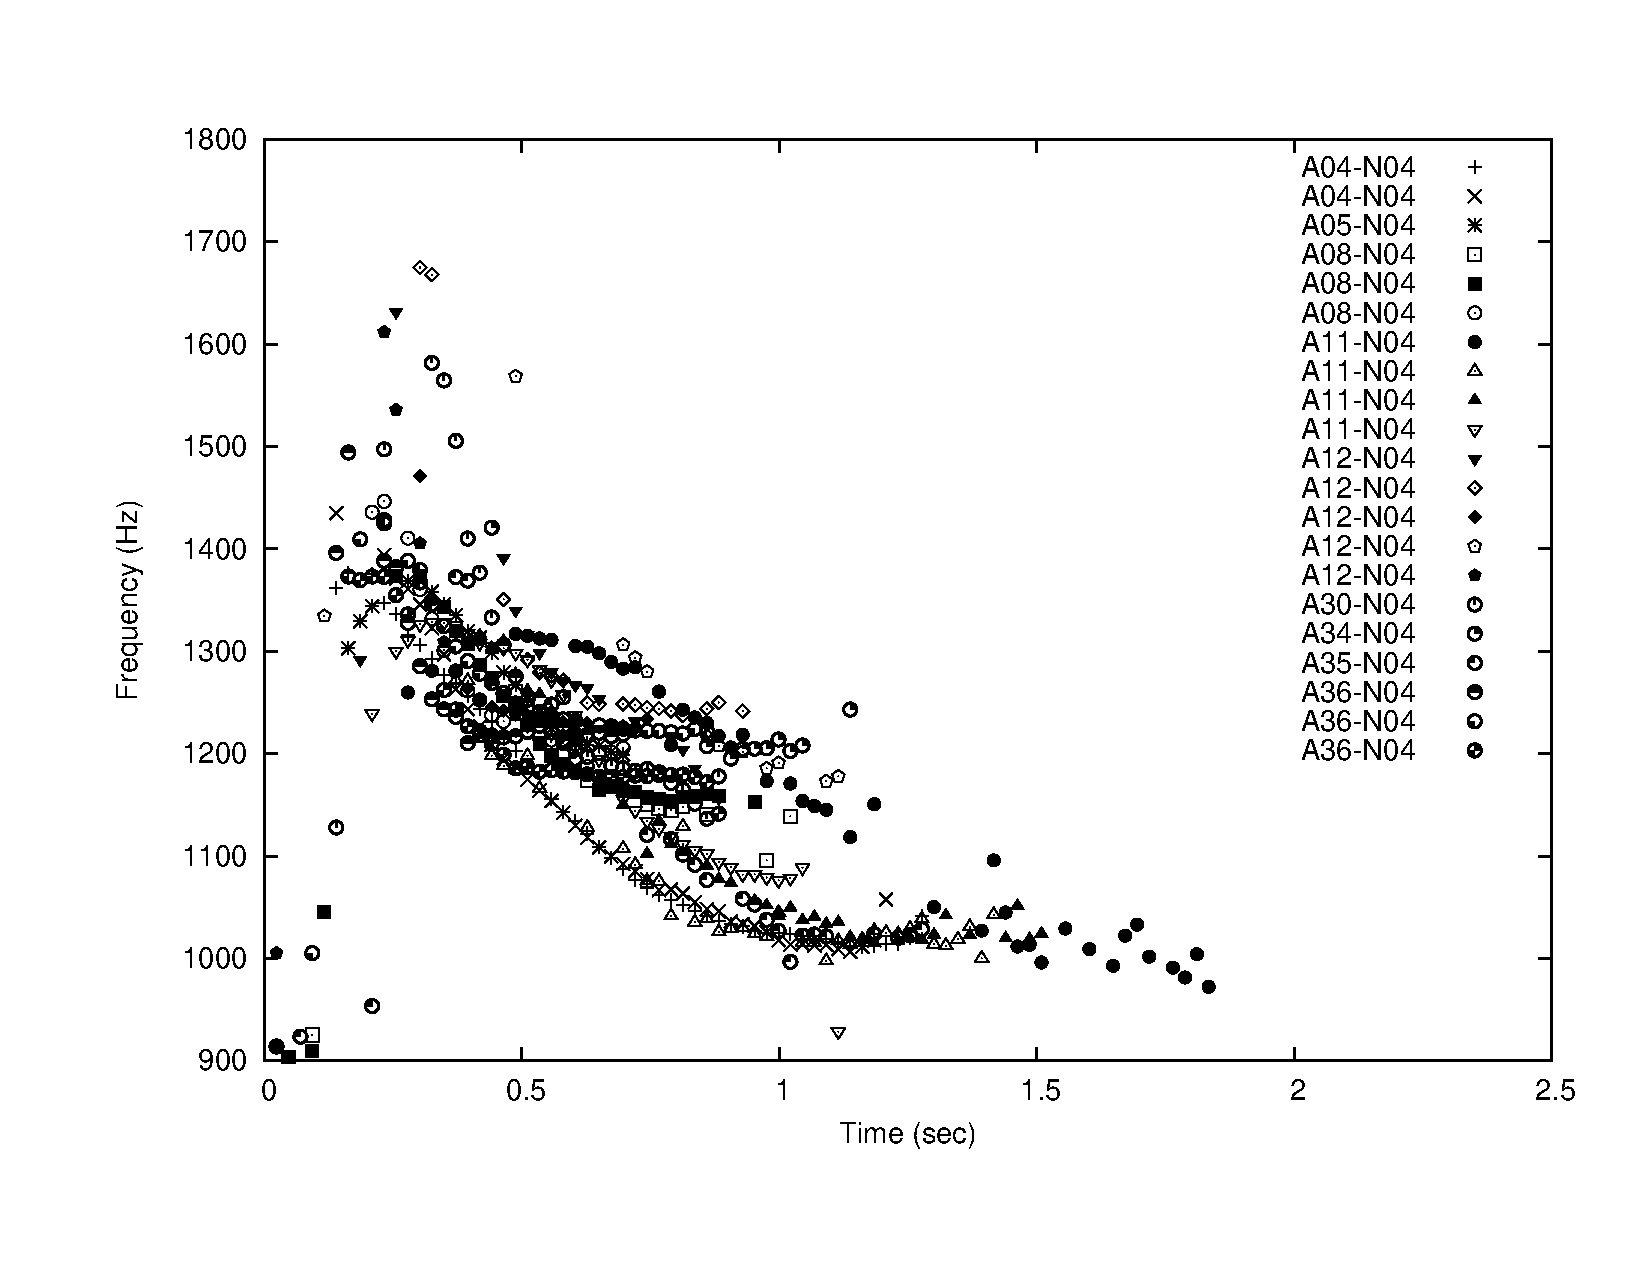
\includegraphics[width=90mm]{images/pitch-N04}
\caption{F0 contour for 21 examples of the N04 call.}
\label{fig:pitch-N04}
\end{figure}

\begin{figure}[h]
\centering
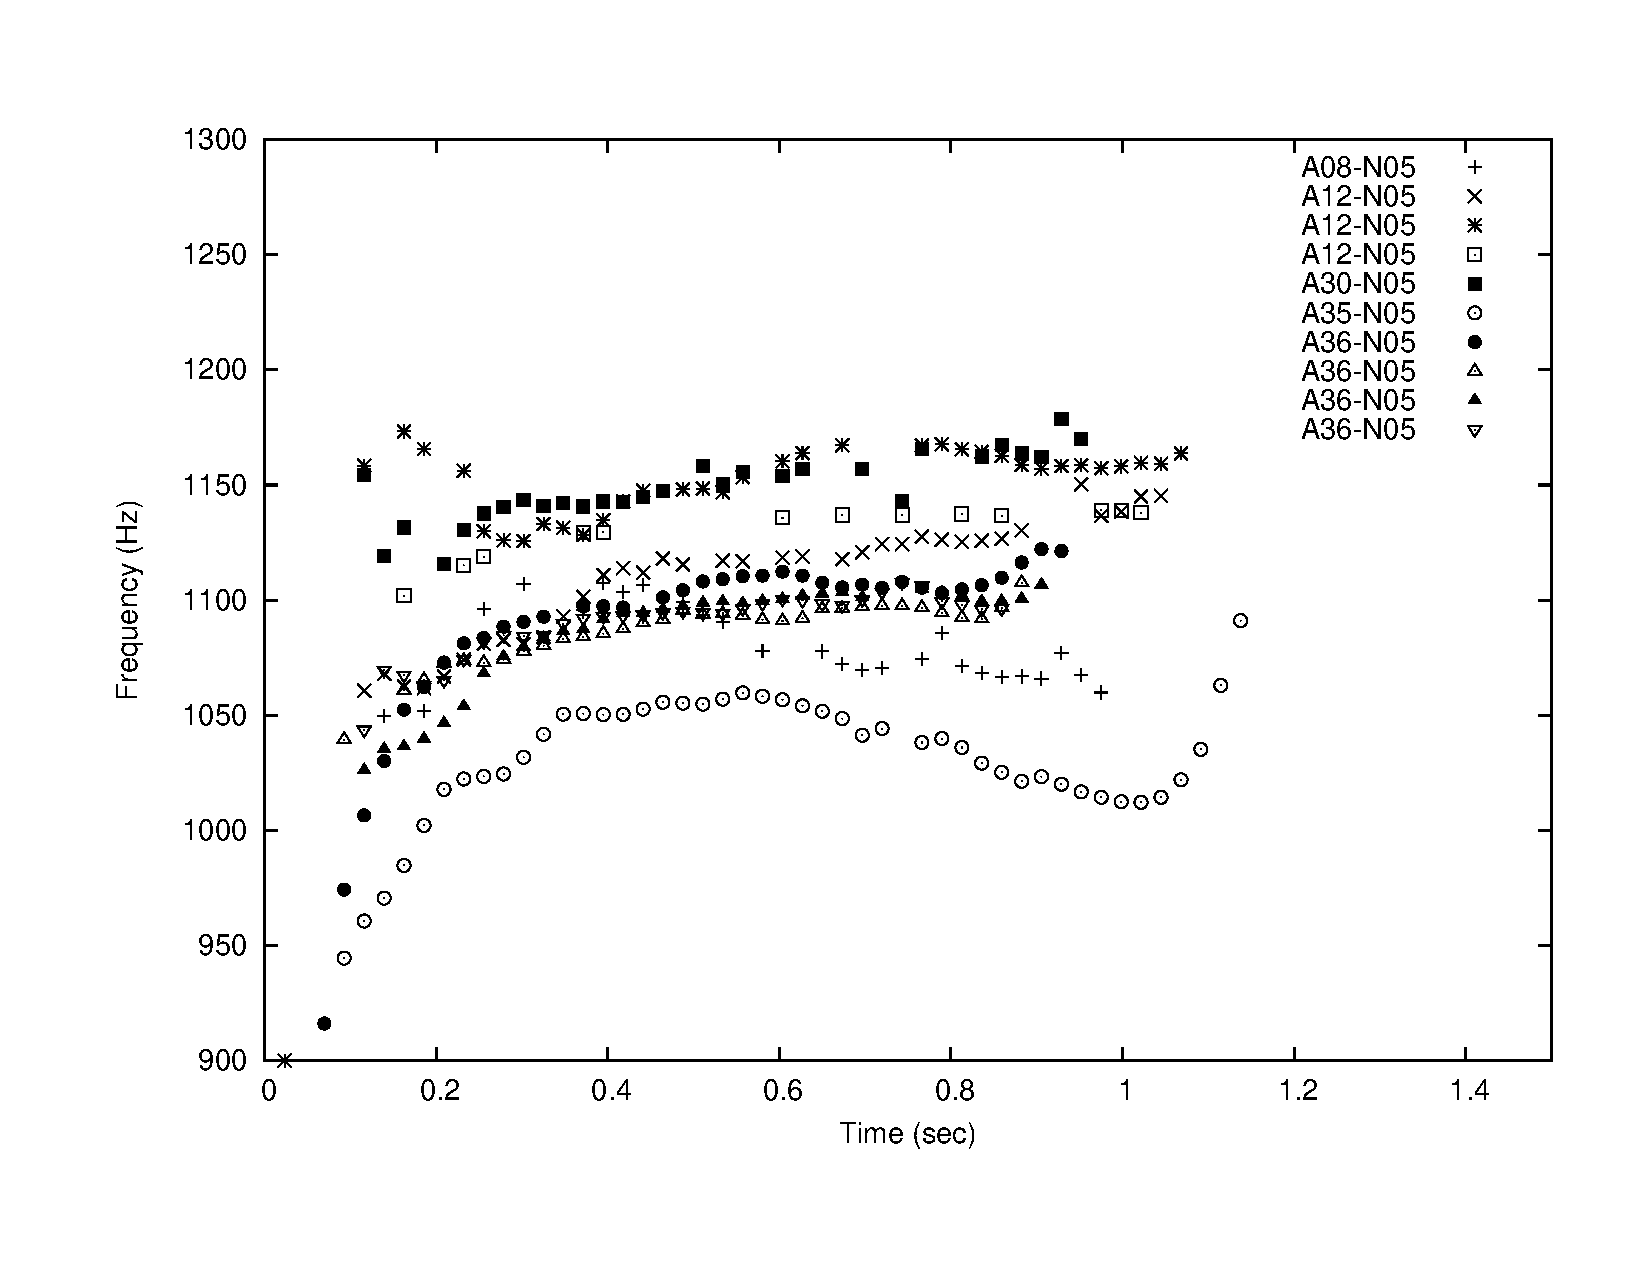
\includegraphics[width=90mm]{images/pitch-N05}
\caption{F0 Contour for 10 examples of N05 call.}
\label{fig:pitch-N05}
\end{figure}

This approach is certainly valid if slope changes within a given
window characterize the signal well and the signal is fairly free of
noise. We therefore have examined SAX for a possible avenue to
transcribe Orca vocalizations. We determined, however, that
considering windowed slope fragments of Orca vocalizations does
produce sequences that are of lower quality than those produced by our
transcription technique which we refer to as FTSQ (Fundamental
Frequency Time Series Quantization).  The FTSQ procedure is outlined
in detail below. We do not provide classification results for SAX
sequences because the majority of SAX sequences were too long in order
to be processed by our dynamic programming based alignment algorithm
and hence a direct comparison can't be impartial. Further, we observed
that the fundamental frequency of Orca vocalizations carries a lot of
information, that is, it seems to be stable, and within a certain
range that is unique to a large portion of the vocalizations in our call
catalog. Since SAX is normalizing the signal slope within a sliding
window it cannot take advantage of this important feature.

\subsection{Signal Pre-processing and FTSQ}

Fundamental Frequency Time Series Quantization is a time series
quantization approach that transcribes an audio time series based on
an estimate of it's fundamental frequency ($F_0$).

In general it is not feasible to analyze Orca vocalizations as a raw
time series, since these signals are a complex mixture of sinusoids and
noise (see Figure \ref{fig:audio_raw}).  Figure \ref{fig:freqspec}
shows a spectrogram representation of the N01 and N09 Orca
vocalizations.  When comparing Figures \ref{fig:audio_raw} and
\ref{fig:freqspec} it is easy to see that the frequency components of
the audio signal reveals much more about the structure of the signal
than a raw audio time series by itself.

\begin{figure}[h]
\centering
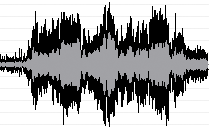
\includegraphics[width=0.4\columnwidth]{images/audio_raw}
\caption{Raw audio signal of Orca vocalization N01.}
\label{fig:audio_raw}
\end{figure}
\begin{figure}[h]
\centering
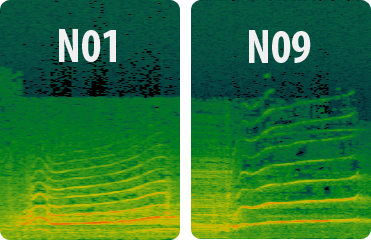
\includegraphics[width=0.60\columnwidth]{images/freq_N01N09.png}
\caption{Frequency spectrum of Orca vocalizations N01 and N09.}
\label{fig:freqspec}
\end{figure}

Quantizing the fundamental frequency of an audio signal is am approach that makes 
use of the underlying structure in the frequency bands of the audio signal.
Loosely speaking one may think of the fundamental frequency as the pitch of a sound signal.
For our FTSQ technique we use Yin \cite{Cheveigne2002} a robust fundamental frequency 
estimation algorithm developed by Cheveigne et al.
Processing the audio waveform from Figure~\ref{fig:audio_raw} with Yin yields the 
fundamental frequency (in octaves relative to 440 Hz) shown in the top plot of Figure \ref{fig:yin}.
The two plots below the fundamental frequency show the aperiodicity and the
period-smoothed instantaneous power of the signal; they give estimate in the 
confidence on the approximation of $F_0$ and are used to identify meaningful
regions of interest within the $F_0$ signal.
\begin{figure}[h]
\centering
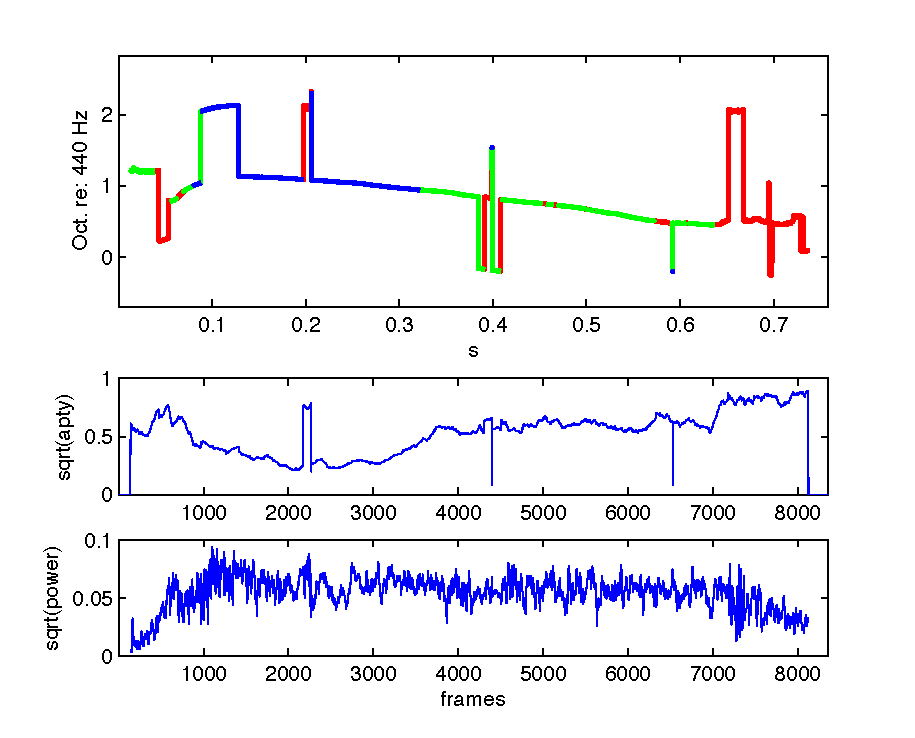
\includegraphics[width=\columnwidth]{images/yin}
\caption{Frequency spectrum of Orca vocalizations N01 and N09}
\label{fig:yin}
\end{figure}


A further issue that is encountered commonly in the process of
determining a pitch contour for an audio recording is the optimization
of all the parameters of the pitch detection algorithm to perform well
on the particular dataset that is being used.  There are many such
parameters for each different algorithm, the important ones in the Yin
algorithm include the window size and hop size of the FFT, the high
and low frequency cutoffs, the high and low frequencies around which
the pitches will be wrapped using modulo arithmetic, the tolerance of
the Yin algorithm which determines which peaks in the autocorrelation
will be used for the pitch determination, the window size for the
median filter, and the number of histogram bins in which to divide the
frequency range into.  In our previous work, this was done by hand by
plotting points using MATLAB or Gnuplot, which can be a long and
labour intensive process.

For this project, we added custom visualization tools to our OpenMIR
platform to view the original audio as a spectrogram, to allow the
user to listen to this audio, to show a pitch contour with dynamic
controls over these various parameters, and an energy display that
shows the RMS energy of the audio signal.  This interface is shown in
Figure \ref{fig:openmir}.  This software allowed us to quickly
iterate over a large number of parameters, and to determine the
optimal parameters for the Yin algorithm.  The most important of these
was the median filter size, and a median filter of size 11 is shown in
Figure \ref{fig:openmir}.

\begin{figure}[t]
\centering
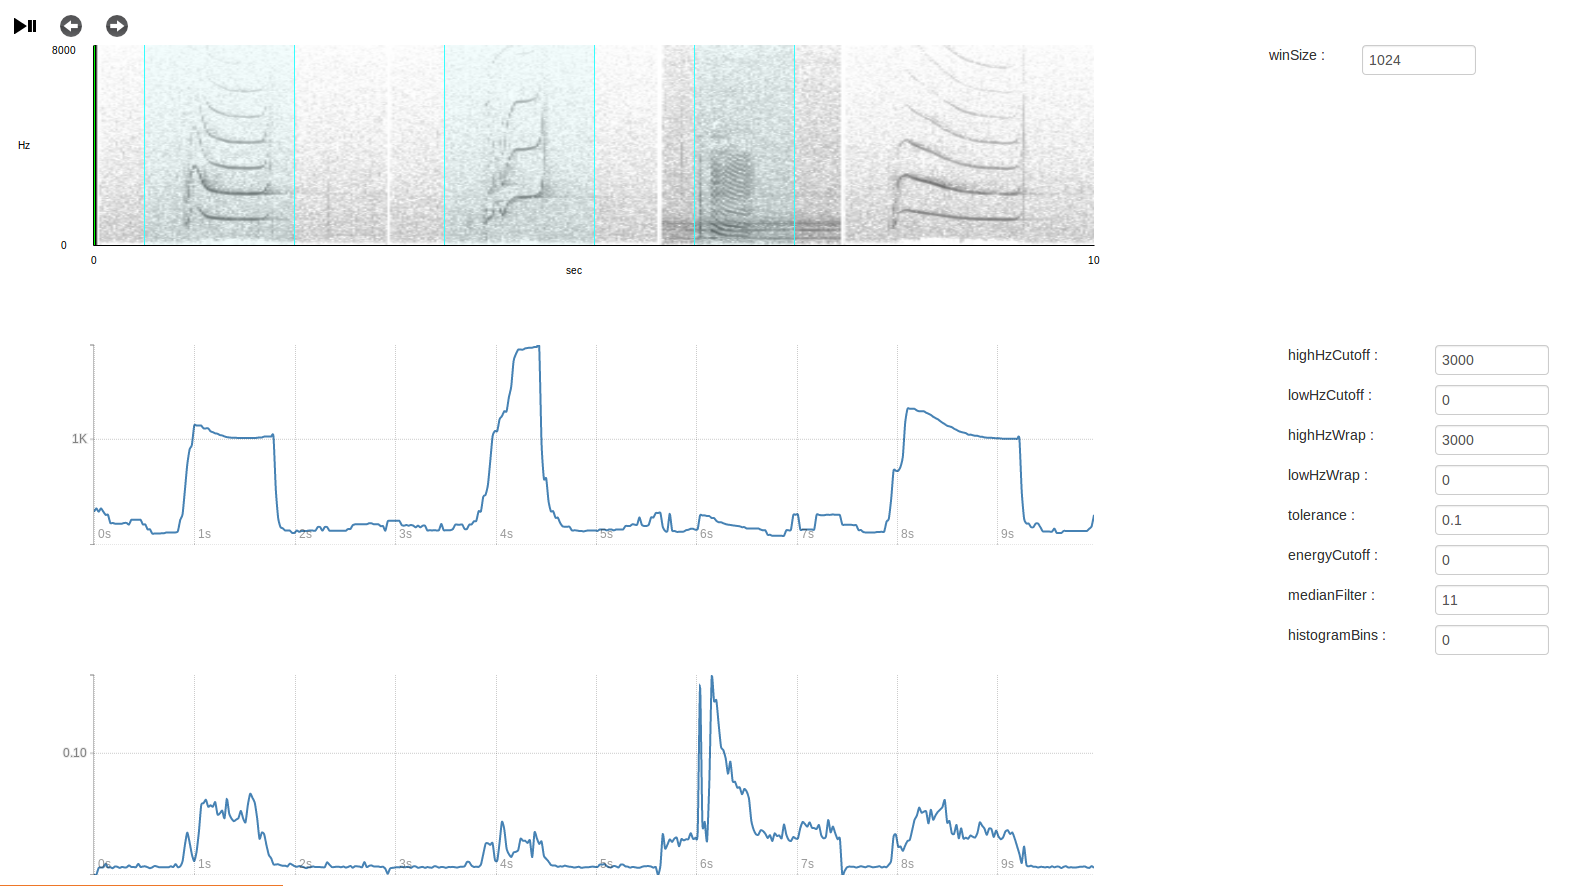
\includegraphics[width=\columnwidth]{images/openmir}
\caption{Spectrogram, pitch and RMS view of a small portion of the Orchive
catalog viewed with the OpenMIR interface. }
\label{fig:openmir}
\end{figure}

\subsubsection{Octave Errors}
The output of Yin does not always give a proper estimate of $F_0$.
Indeed, the $F_0$ signal in Figure \ref{fig:yin} displays several
estimation errors that we herein refer to as \emph{octave errors}.
Octave errors manifest themselves as sudden jumps in a multiple of the
core $F_0$ frequency. Figure \ref{fig:yin} displays multiple octave
errors the first one at about 0.1 seconds. When quantizing the $F_0$
signal into a letter representation over a finite alphabet. Octave
errors result in mis-mapped letters in the output sequence. To a
certain degree we are able to handle octave errors by crafting a
custom substitution matrix in our sequence alignment
algorithm. However, doing so ultimately lowers the confidence in our
alignment score and might confuse legitimate frequency jumps with
octave errors and as a result would not penalize mismatches
appropriately. Therefore, we have developed a technique that can
automatically correct for the majority of octave errors and as a net
effect produces a more accurate letter representation.

We first run the $F_0$ signal obtained from Yin through a median filter, 
which smoothes the signal and eliminates small transients that occur due
to noise in the original signal. We then threshold the aperiodicity and the
period-smoothed instantaneous power to obtain $F_0$ signal regions at which
the $F_0$ signal is estimated with high confidence. After down-sampling the
signal we obtain the representation shown in Figure
\ref{fig:clean_yin}.

\begin{figure}[h]
\centering
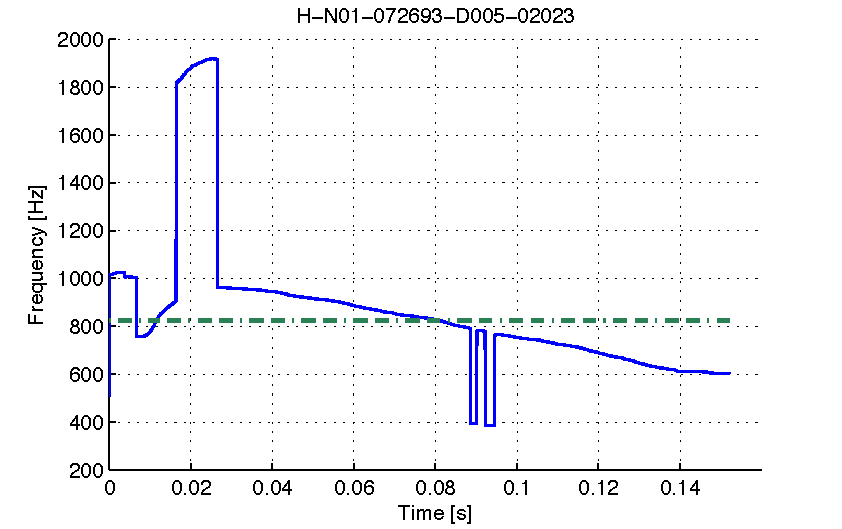
\includegraphics[width=\columnwidth]{images/yin_clean}
\caption{Thresholded and down-sampled $F_0$ signal of a N01 call.}
\label{fig:clean_yin}
\end{figure}

The green line represents the median of the original $F_0$ signal
drawn in blue. The octave errors are clearly identifiable as such in
Figure \ref{fig:octave_yin} which shows versions of the $F_0$ signal
one octave above (purple) and on octave below (red) the original
(blue).  $F_0$ signal. To correct for octave errors we simply piece
the portions of the three versions of the $F_0$ signal together
according to which ever signal is closest to a slightly upwards biased
median of the original signal (blue). This yields the black $F_0$
curve wich shows the now automatically corrected version of the $F_0$
signal.
\begin{figure}[h]
\centering
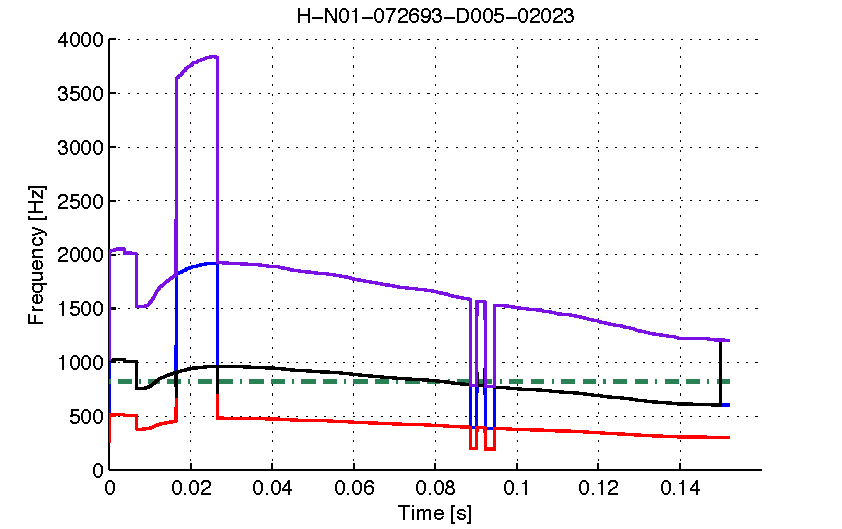
\includegraphics[width=\columnwidth]{images/octave_fix}
\caption{Octave errors within a $F_0$ signal of a N01 call.}
\label{fig:octave_yin}
\end{figure}

\subsection{Log-Normal Signal Quantization}
When transcribing the $F_0$ signal into a letter representation suitable 
for sequence alignment tools it is natural to ask how these letters should be
assigned over the range of possible $F_0$ frequency values. A naive approach
would be to map $F_0$ frequencies to letters in a linear fashion. However, while
this approach does work well in practice, we investigated if a non-linear mapping
might potentially be more appropriate. For this purpose we plotted
the distribution of $F_0$ frequencies over time for the whole catalog of
Orca vocalizations in Figure \ref{fig:freq_dist}. The dynamic range of
$F_0$ incorporates frequencies from about 80 to 2400Hz, with three high density bands
at around 250, 700 and 1200Hz. Ideally one would therefore quantize the $F_0$ signal
using a three-modal distribution. However, for simplicity we chose a log-normal 
distribution (see Figure \ref{fig:log_norm}), which provides us with a fine resolution
for the more common $F_0$ frequencies and quantizes high $F_0$ frequencies at a coarser level.
\begin{figure}[h]
\centering
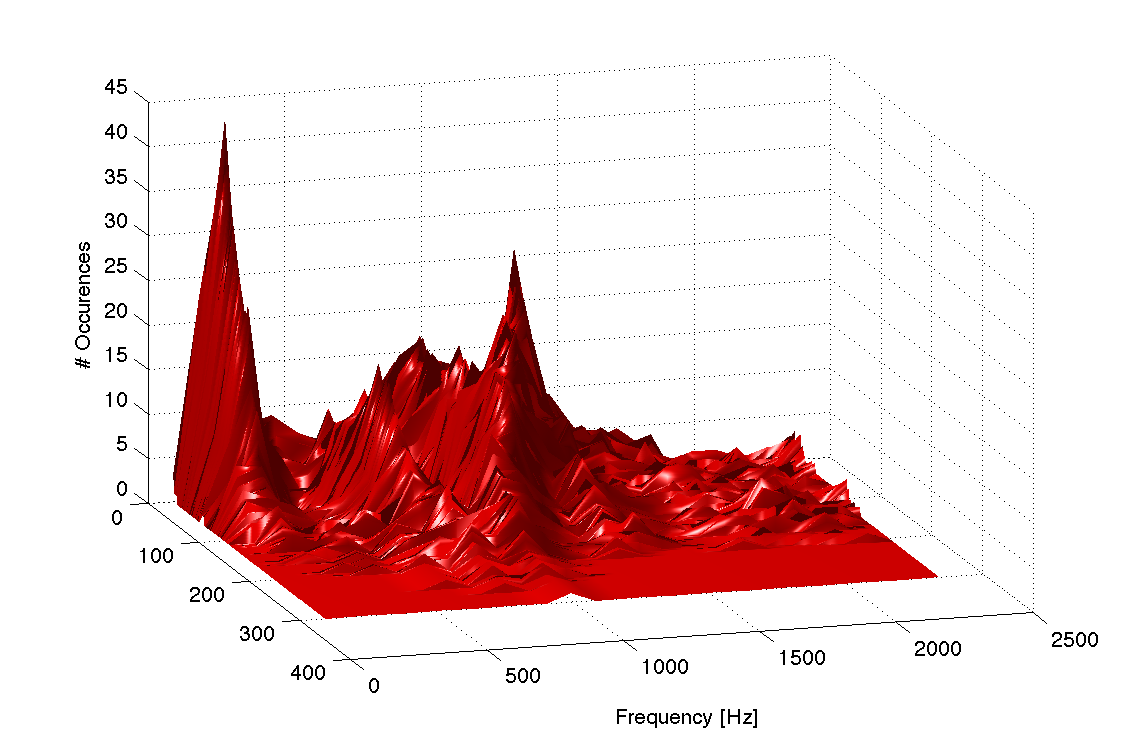
\includegraphics[width=\columnwidth]{images/freq_dist}
\caption{Distribution of $F_0$ frequencies of call catalog.}
\label{fig:freq_dist}
\end{figure}

\begin{figure}[h]
\centering
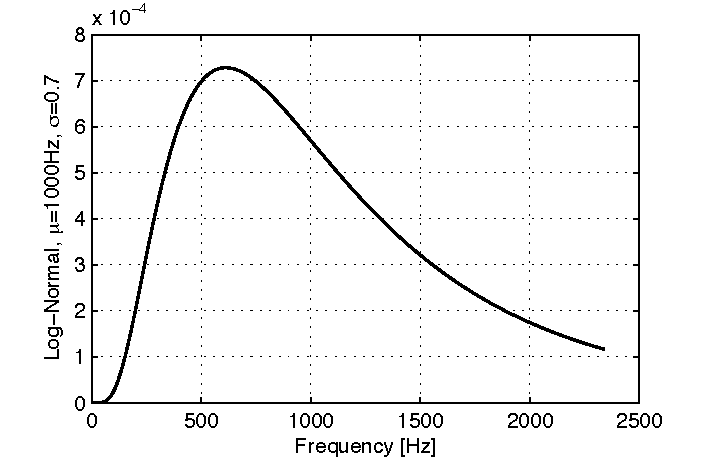
\includegraphics[width=0.7\columnwidth]{images/log_norm}
\caption{Log-normal distribution for quantization}
\label{fig:log_norm}
\end{figure}

The result of log-normal quantization of the $F_0$ trace in Figure
\ref{fig:octave_yin} is provided in Figure
\ref{fig:letter_curve}. Finally, the resulting letter sequence is
given by \texttt{LLHHJJKKKKKKKKKKKKJJJJJJJII--IIIIIHHHHHHHGGGGGFFFFFF}
which can readily be consumed by a dynamic programming sequence
alignment algorithm.

\begin{figure}[h]
\centering
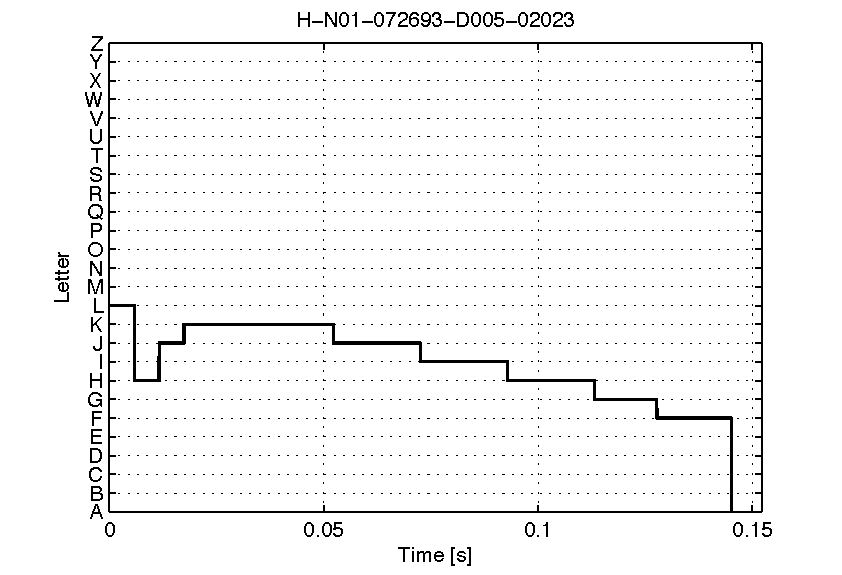
\includegraphics[width=\columnwidth]{images/letter_curve}
\caption{$F_0$ signal of N01 call quantized to a finite alphabet}
\label{fig:letter_curve}
\end{figure}

\begin{table}
\centering
\begin{tabular}{|c|c|} 
\hline
Data Set                         &  Global Accuracy  \\
\hline
Original                         &              64\%  \\
Octave Removal - Linear          &              81\%  \\
Octave Removal - NonLinear 900   &              80\%  \\
Octave Removal - NonLinear 1200  &              81\%  \\
J48                              &              58\%  \\
Naive Bayes                      &              65\%  \\
SVM                              &              75\%  \\
\hline
\end{tabular}
\caption{Global accuracy for different methods of converting a Yin
  pitch contour into an alphabet using FTSQ}
\label{table:performance}
\end{table}


\begin{table}
\centering
\begin{tabular}{|c|c|} 
\hline
 Call  &  Accuracy  \\
\hline
 N47   &     0.400  \\
 N01   &     0.969  \\
 N12   &     0.583  \\
 N05   &     0.785  \\
 N04   &     1.000  \\
 N03   &      0.75  \\
 N09   &     0.772  \\
\hline
\end{tabular}
\caption{Global accuracy for different call types using Octave Removal
  NonLinear 1200 parameters with the FTSQ algorithm.}
\label{table:performance}
\end{table}

\section{Alphabetic Sequence Representation}

In order for sequence comparison algorithms to work well, it is
necessary that the combination of the letters and the scoring matrix
are compatible and output meaningful results.  In the two sections
below, we show the result of quantizing the signal using the nonlinear
histogram approach for two of the more common calls vocalized by
A-clan Northern Resident whales.  The first is the very common N4
call, which consists of a quick up swing in pitch, followed by a
downswing and then a constant tone.  In it we can clearly see long
regions of the repeated letters, P,O,N,M,L,K.  Even from a quick
visual inspection these repeated letters show that our method of
converting frequencies into a discrete alphabet is promising.

{\tiny
\begin{verbatim}
N04 A04 HIKNOOOOOPPPPOOOOOOOOOOOONNNNNNNNNNNNMMMMMMMMMMMMLLLLLLLLLLLLLLLLLLKKKKKKKKKKKKKKK
N04 A04 IJNOPPPPPPPPPPPOOOOOOOOONNNNNNNNMMMMMMMMMMMMMMLLLLLLLLLLLLLLLLLLLLLLKKKKKKKKKKKKKK
N04 A05 NLKLMNOOOOOOOOOOOOOOOOOOOOOOOOOONNNNNNNNNNNNNNNNNNNNMHGQ
N04 A08 RILMNNOOOOOOOOIIOOOOOOOOOOONNNNNNNNNNNNNNNNNNNNNMMMMMMMMMMMMMMMMMMMMMLLLLLLLMLLLLL
N04 A08 SIIJJKNPQQRPIIOOOOOOOONNNNNNNNNNNNNNMMMMMMMMMMMMMMMMMMMMMMMMMMDCCCMMM
\end{verbatim}
}

Even more promising were the results for another call, N5, which
consists of a constant tone.  These calls are from the A36 matriline
of orcas, which now consists of only two whales, the brothers A37 and
A46, although the grandmother whale, A12 often now associates with
this matriline after A34, her daughter's matriline, grew large in
size.  From these calls, we can see that the frequency represented by
the letter L is very constant throughout the entire call, and is a
clear indication that this is an N5 call.

{\tiny
\begin{verbatim}
N05,A36,A36-N05-070806-D012-13913,IIJJJKKKKKLLLLLLLLLLLLLLLLLLLLLLLLLLLLLLLLLLLLLLLLLLLLLL
N05,A36,A36-N05-070806-D012-13917,JJJKKLLFLLLLLLLLLLLLLLLLLLLLLLLLLLLLLLLLLLLLLLLLLLLLLLLL
N05,A36,A36-N05-070806-D012-13921,IIJJKKKKKKKKKLLLLLLLLLLLLGLLLLLLLLLLLLLLLLLLLLLLLLLLLLLL
N05,A36,A36-N05-071506-D017-11311,IQHJKLLLLLLLLLLLLLLLLLLLLLLLLLLLLLLLLLLLLLLLLLLLLLLLLLLL
\end{verbatim}
}
